\graphicspath{{Ch5_VHqqbb/figures/}}

\chapter{$VH \rightarrow q\bar{q}^{(\prime)}b\bar{b}$}
\dots

\section{Theoretical Motivation/Overview}
\dots


\begin{figure}
	\centering
	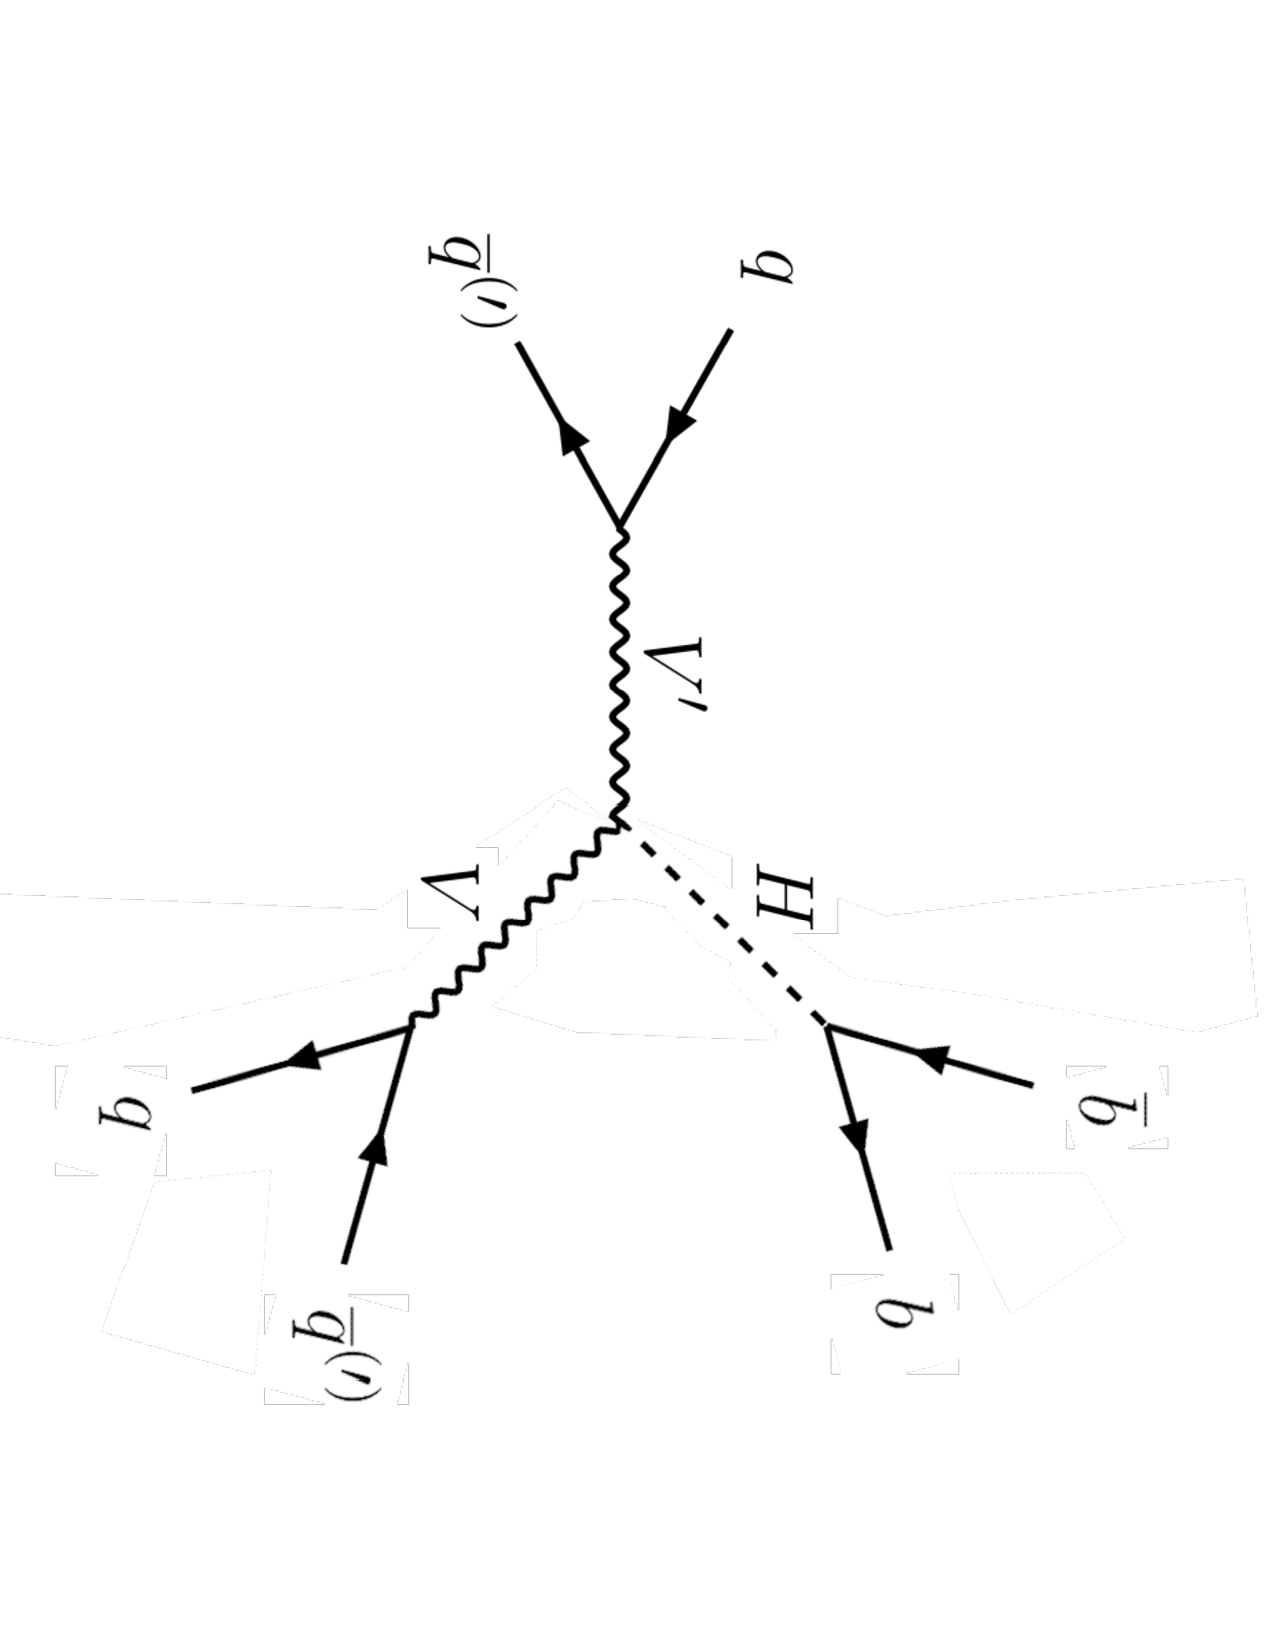
\includegraphics[width=0.75\textwidth,angle=90,origin=c]{feynman_diagram_VHqqbb}
	\caption{}
	\label{fig:feynman_diagram_VHqqbb}
\end{figure}

\section{Analysis Strategy}
\dots

\section{Data and Simulated Samples}
\dots
\subsection{Data}
\dots
\subsection{Signal}
\dots
\subsection{Backgrounds}
\dots
\subsubsection{QCD}
\dots
\subsubsection{$V$+jets}
\dots
\subsubsection{t$\bar{t}$}
\dots

\section{Event Selection}
\dots
\subsection{Trigger Requirements}
\dots
\subsection{Object Selection}
\dots
\subsection{Boson Tagging}
\dots
\subsection{Control/Validation Regions}
\dots

\section{BDT Re-Weighting}
\dots

\section{Background Fitting}
\dots

\section{Statistical Method}
\dots

\subsection{Overview}
% cite hypothesis testing by gregory schott from 'data analysis in high energy physics' textbook
In the absence of a discovery, The primary goal of this thesis is to place limits on a particular parameter of the HVT model: the production cross section.
This type of statistical inference is often called \textit{parameter estimation}, but more fittingly in this case, \textit{parameter constraint}. 
We begin with two hypotheses: the null hypothesis $H_0$ and the alternative hypothesis $H_1$.
In the context of a search for new physics $H_0$ is often referred to as the \textit{background-only hypothesis}, under the assumption that only Standard Model processes contribute to the observed data.
The complementary $H_1$ hypothesis, known as the \textit{signal-plus-background hypothesis}, includes the contribution of the new physics signal in addition to the Standard Model background.
For this analysis $H_1$ is in fact a family of hypotheses because both the resonance mass and production cross section are explored via continuous parameters of the HVT model.

The fundamental tool of frequentist hypothesis testing is the \textit{test statistic}, which is used to make quantitative statements about the data and its relationship to $H_0$ and $H_1$.
Given some measurements $X$, a test statistic $t(X)$ can be any (scalar, for our purposes) function.
There are, of course, desirable properties that constrain the types of functions that should be used as the test statistic.
The final conclusions about the hypotheses are based upon the comparison of the observed value of $t(X)$ to some pre-determine \textit{critical region}.
In our case of parameter constraint, the critical region is defined by a single cut value $t_c$.
It is assumed that $t$ tends to have smaller values under $H_0$ and larger values under $H_1$, and thus the critical region is $t > t_c$.

The next ingredient needed is the probability density function of $t$ under a given hypothesis $H$, $g(t|H)$.
% mention Wilks and Wald theorems

Two important quantities are defined via $g$,
\begin{align}
    \alpha &\equiv \int_{t_c}^{+ \infty} g(t|H_0)dt \\
    \beta &\equiv \int_{-\infty}^{t_c} g(t|H_1)dt
\end{align}
The probability that to reject the background-only hypothesis ($H_0$) even though it is true is given by $\alpha$.
The probability that to reject the signal-plus-background hypothesis ($H_1$) even though it is true is given by $\beta$.
An ideal test statistic will minimize $\beta$ for a given $\alpha$.
Often $\alpha$ is referred to as the \textit{significance level} of the test and $1-\beta$ is called the \textit{power} of the test.
For a new physics search $\alpha$ must of necessity be quite small and is typically chosen to be 5\%.
It is important to note at this point that the values of both $\alpha$ and $\beta$ are independent of the observed data $X$, rather they indicate something about the quality and characteristics of the statistical method that will eventually be applied to data.

There is some freedom allowed in the choice of $t(X)$, but when dealing in so-called \textit{simple hypotheses}, as we are here, the Neyman-Pearson lemma states that the \textit{likelihood ratio} is the most powerful test for any given significance level $\alpha$.

\subsection{CLs Method}


\section{Systematic Uncertainties}
